

\section{Linear algebraic mechanisms behind sink tokens}

\tianyu{Massive tokens are not necessarily sink tokens in OOD?}

\yub{better title?}

\yub{In each subsection, we give a set of plots (in 1 - 2 lines), and give some explanation. If there is some further studies that naturall come after the initial set of plots, we give another set of plots.}

Throughout the rest of this section, we use LlaMa2-7B~\citep{touvron2023llama}.

\subsection{Birth of sink tokens}

\paragraph{How are sink tokens produced?}
% ~\yub{mostly done.}

\cref{fig:mlp1} shows that $\MLP_1$ produces the sink tokens, i.e. makes certain tokens have massive norms.


LlaMa's MLP layer is defined by three weight matrices $\sets{\Wgate, \Wdown, \Wup}$~\yub{dimensions} with the SwiGLU activation~\citep{shazeer2020glu}:
\begin{align}
    f_{\mlp}(\bh) = \Wdown \paren{ \silu\paren{ \Wgate\bh } \odot \paren{\Wup\bh} }.
\end{align}
Above, $\silu(t) \defeq t\cdot \sigmoid(t)$ denotes the SiLU (or Swish) activation~\citep{ramachandran2017searching}.

\begin{figure}[H]
\centering
\begin{minipage}{.32\textwidth}
\centering
    % \subcaption{{\footnotesize BLAH}}\label{fig:11}
    %\vspace{-.7em}
    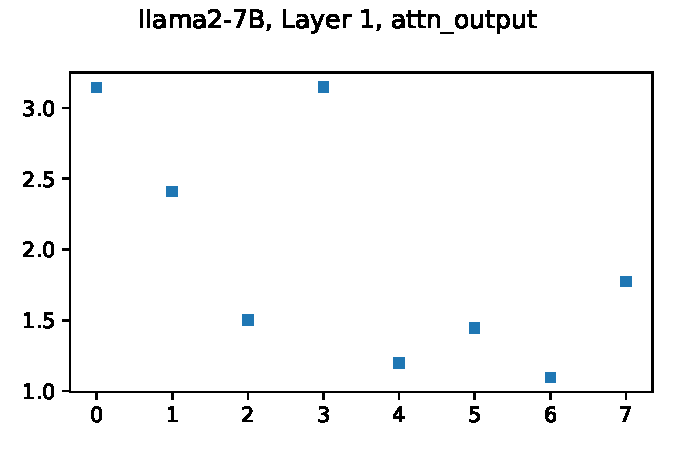
\includegraphics[width=0.95\textwidth]{Figures/Summer/layer_1_attn_output.pdf}
\end{minipage}
% \hfill
\begin{minipage}{.32\textwidth}
    \centering
    % \subcaption{{\footnotesize BLAH}}\label{fig:12}
    %\vspace{-.7em}
    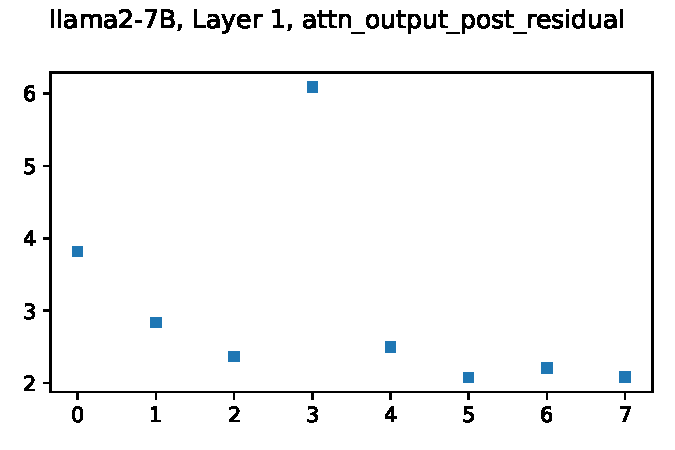
\includegraphics[width=.95\textwidth]{Figures/Summer/layer_1_attn_output_post_residual.pdf}
\end{minipage}
% \hfill
% \begin{minipage}{.24\textwidth}
%     \centering
%     \subcaption{{\footnotesize BLAH}}\label{fig:13}
%     %\vspace{-.7em}
%     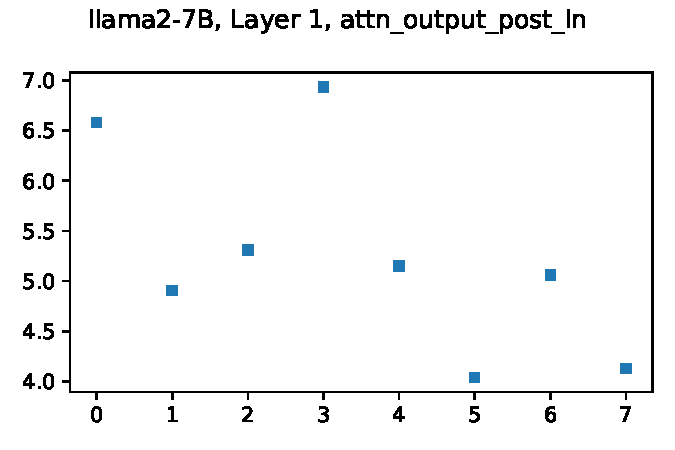
\includegraphics[width=.95\textwidth]{Figures/Summer/layer_1_attn_output_post_ln.pdf}
% \end{minipage}
\begin{minipage}{.32\textwidth}
    \centering
    % \subcaption{{\footnotesize BLAH}}\label{fig:14}
    %\vspace{-.7em}
    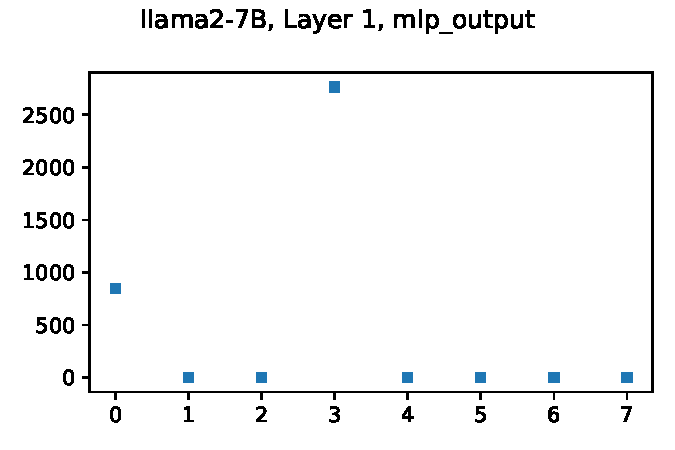
\includegraphics[width=.95\textwidth]{Figures/Summer/layer_1_mlp_output.pdf}
\end{minipage}
\caption{
\small
Sink tokens (token 0 and token 3) are produced by $\MLP_1$. Sentence: ``Summer is warm. Winter is cold.''
\yub{maybe a better illustration is to track the evolution of all 8 tokens, one on each curve, x axis is the module name (along forward pass), y axis is norm.}
}
\label{fig:mlp1}
\vspace{-1em}
\end{figure}

% Group of plots for $\MLP_1$. Plot 0: Narrow it down to MLP1. Plot 1: Some flowchart. Plot 2 (maybe with one other plot that shows the shape of $W3[:, 7890]$): How massive tokens activate the $W_{\{1,2\}}[7890, :]$, and how $W3[:, 7890]$ produces massive entries at $1415, 2533$.


\begin{figure}[H]
\centering
\begin{minipage}{.32\textwidth}
\centering
    \subcaption{{\footnotesize Histogram of $\sets{\ltwos{\Wgate[i, :]}}_{i}$}}\label{fig:w1-norm}
    %\vspace{-.7em}
    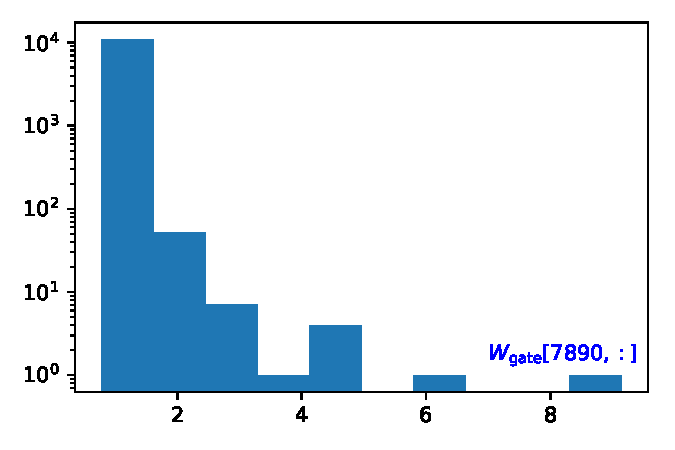
\includegraphics[width=0.95\textwidth]{Figures/Summer/w1_norm_hist.pdf}
\end{minipage}
% \hfill
\begin{minipage}{.32\textwidth}
    \centering
    \subcaption{{\footnotesize $\<\bh_j, \Wgate[i, :]\>$}}\label{fig:corr-w1}
    %\vspace{-.7em}
    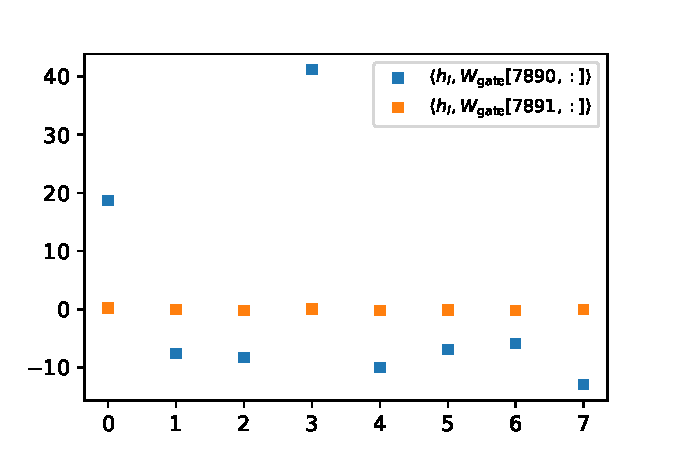
\includegraphics[width=.95\textwidth]{Figures/Summer/corr_with_w.pdf}
\end{minipage}
% \hfill
% \begin{minipage}{.24\textwidth}
%     \centering
%     \subcaption{{\footnotesize BLAH}}\label{fig:13}
%     %\vspace{-.7em}
%     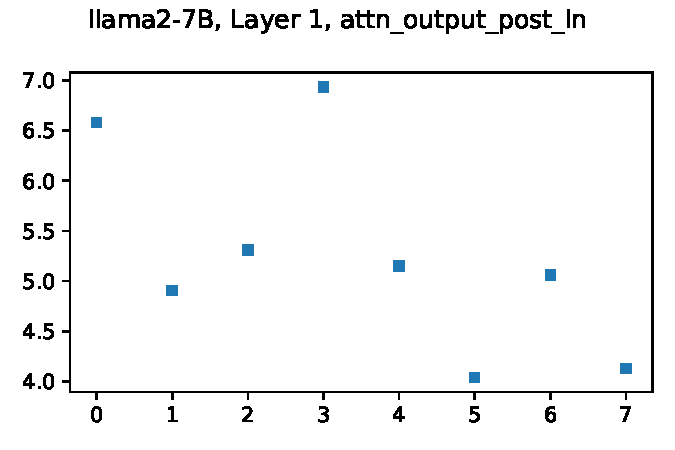
\includegraphics[width=.95\textwidth]{Figures/Summer/layer_1_attn_output_post_ln.pdf}
% \end{minipage}
\begin{minipage}{.32\textwidth}
    \centering
    \subcaption{{\footnotesize $\Wdown[:, i]$}}\label{fig:w3}
    %\vspace{-.7em}
    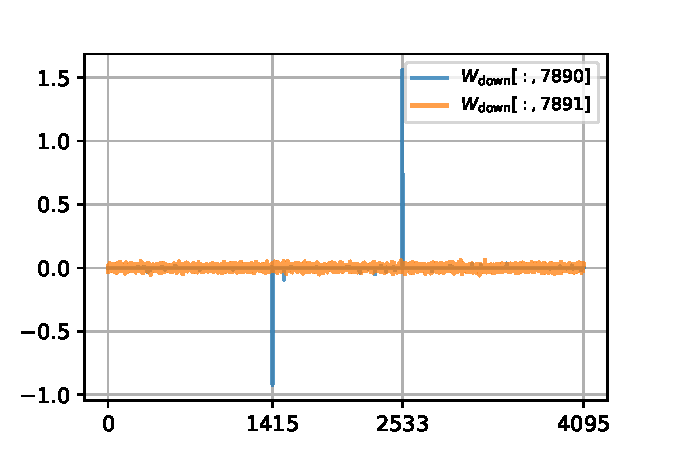
\includegraphics[width=.95\textwidth]{Figures/Summer/w3.pdf}
\end{minipage}
\caption{
\small
Mechanisms of $\MLP_1$. (a) Neuron 7890 has the largest norm among all neurons in $\Wgate$. (b) $\Wgate[7890, :]$ has large positive inner products with sink tokens, and large negative inner products with non-sink tokens. (c) $\Wdown[:, 7890]$ has large entries at $[1415, 2533]$-th coordinate.
Sentence: ``Summer is warm. Winter is cold.''
}
\label{fig:special-neuron}
\vspace{-1em}
\end{figure}

\textbf{What does the special neuron tell us?} By computing the correlations of hidden states and $\Wgate[7890, :]$, we can detect important sub-layers that contribute to the massive tokens.

\begin{figure}[H]
\centering
\begin{minipage}{.24\textwidth}
\centering
    \subcaption{Layer 0 with ROPE}\label{fig:l0-rope-corr}
    %\vspace{-.7em}
    \includegraphics[width=0.95\textwidth]{Figures/tianyu_tentative/layer0wrope.png}
\end{minipage}
% \hfill
\begin{minipage}{.24\textwidth}
\centering
    \subcaption{Layer 1 with ROPE}\label{fig:l1-rope-corr}
    %\vspace{-.7em}
    \includegraphics[width=0.95\textwidth]{Figures/tianyu_tentative/layer1wrope.png}
\end{minipage}
\begin{minipage}{.24\textwidth}
\centering
    \subcaption{Layer 0 without ROPE}\label{fig:l0-norope-corr}
    %\vspace{-.7em}
    \includegraphics[width=0.95\textwidth]{Figures/tianyu_tentative/layer0norope.png}
\end{minipage}
\begin{minipage}{.24\textwidth}
\centering
    \subcaption{Layer 1 without ROPE}\label{fig:l0-rope-corr}
    %\vspace{-.7em}
    \includegraphics[width=0.95\textwidth]{Figures/tianyu_tentative/layer1norope.png}
\end{minipage}
\caption{
\small
Bar-plots of correlations between hidden states and $\Wgate[7890, :]$.
}
\label{fig:special-neuron}
\vspace{-1em}
\end{figure}


\paragraph{Why does the initial token always become a sink token?}
Our approach is to examine the forward pass of all 32K tokens in LlaMa tokenizer.

% Do all the 32000 tokens get to be attention sinks when placed at the initial position?~\yub{vast majority, but not all.}

\begin{figure}[H]
\centering
\begin{minipage}{.25\textwidth}
\centering
    \subcaption{{\footnotesize Norm after Layer 1}}\label{fig:initial-layer1-norm}
    %\vspace{-.7em}
    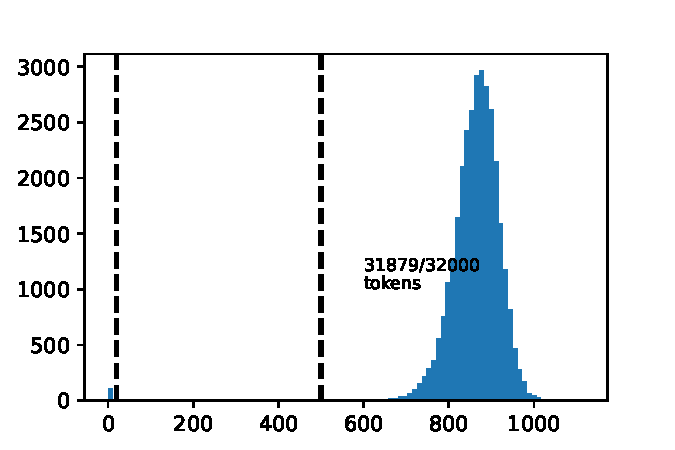
\includegraphics[width=\textwidth]{Figures/initial_token/token_0_layer_1_out_norms.pdf}
\end{minipage}
% \hfill
\begin{minipage}{.25\textwidth}
    \centering
    \subcaption{{\footnotesize Norm of embeddings}}\label{fig:initial-embed-norm}
    %\vspace{-.7em}
    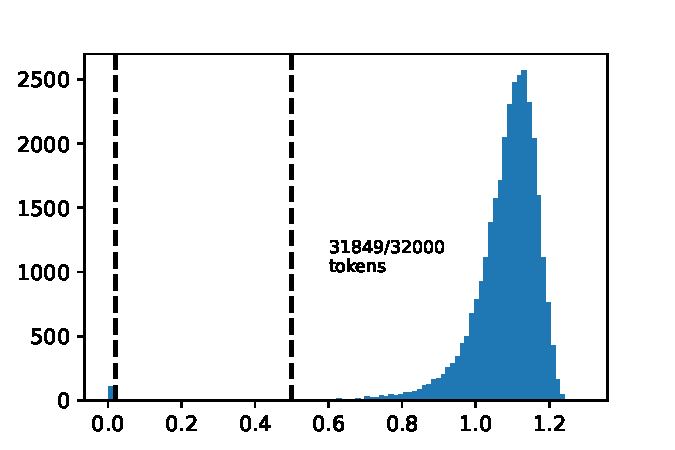
\includegraphics[width=\textwidth]{Figures/initial_token/token_0_embed_norms.pdf}
\end{minipage}
% \hfill
% \begin{minipage}{.24\textwidth}
%     \centering
%     \subcaption{{\footnotesize BLAH}}\label{fig:13}
%     %\vspace{-.7em}
%     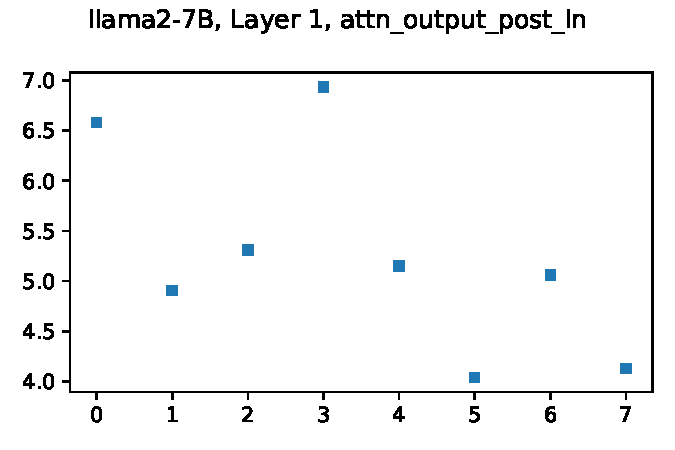
\includegraphics[width=.95\textwidth]{Figures/Summer/layer_1_attn_output_post_ln.pdf}
% \end{minipage}
\begin{minipage}{.48\textwidth}
    \centering
    \subcaption{Inner product with $\bw_\star$}\label{fig:ph}
    %\vspace{-.7em}
    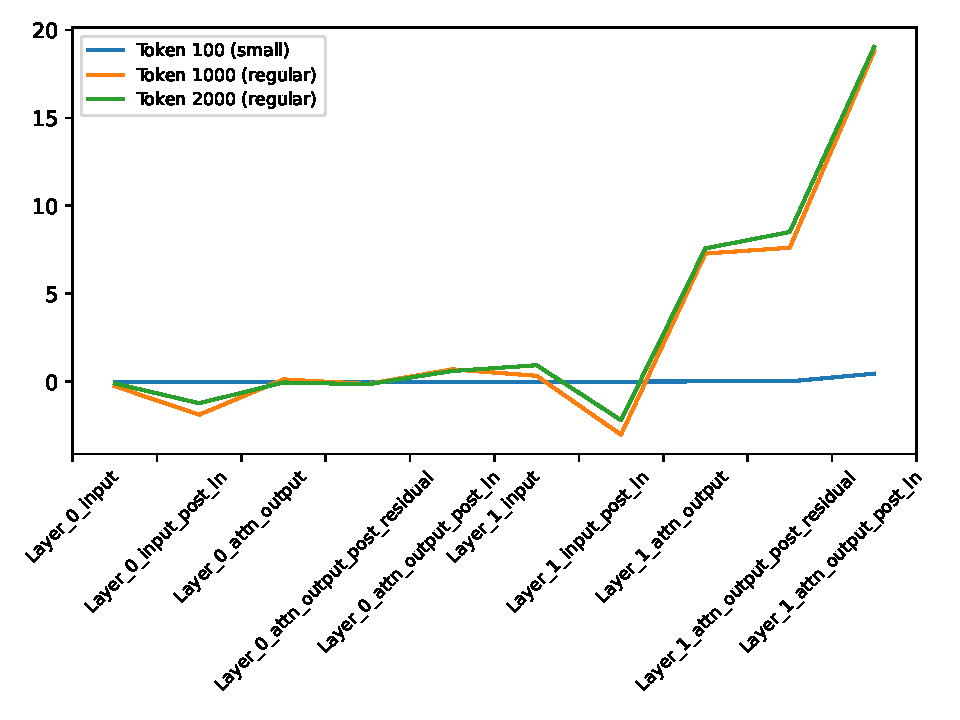
\includegraphics[width=\textwidth]{Figures/initial_token/evolution_initial_token.pdf}
\end{minipage}
\caption{
\small
Evolution of token 0 along the forward pass. Here each sentence just consists of a single token.
}
\label{fig:special-neuron}
\vspace{-1em}
\end{figure}

% \yub{TODO(yub): Evolution of initial token to be aligned with $\bw_\star$. Choose one regular token, and one small token. Also work out a common plot scheme for evolution plots.}

% Plot 1. Out of the 32000 tokens, about 31800 of them gets to be massive when placed at the initial token (maybe use one plot). Plot 2: Evolution of initial token to be aligned with $\bw_\star$.

\yub{TODO(Tianyu): exhaust the list of delimiter tokens (among 32K tokens), defined as any token that becomes massive at non initial locations.}

\paragraph{Which head turns token 0 into sink token?}

\yub{Tianyu has some findings here (Attn1, Head8).}~\yub{Made a plot for Attn1 in~\cref{fig:attn1-heads-rope}.}

Head 8 in $\Attn_1$ is the main symmetry breaker here. See~\cref{fig:attn1-heads-rope}.

\begin{figure}[H]
    \centering
    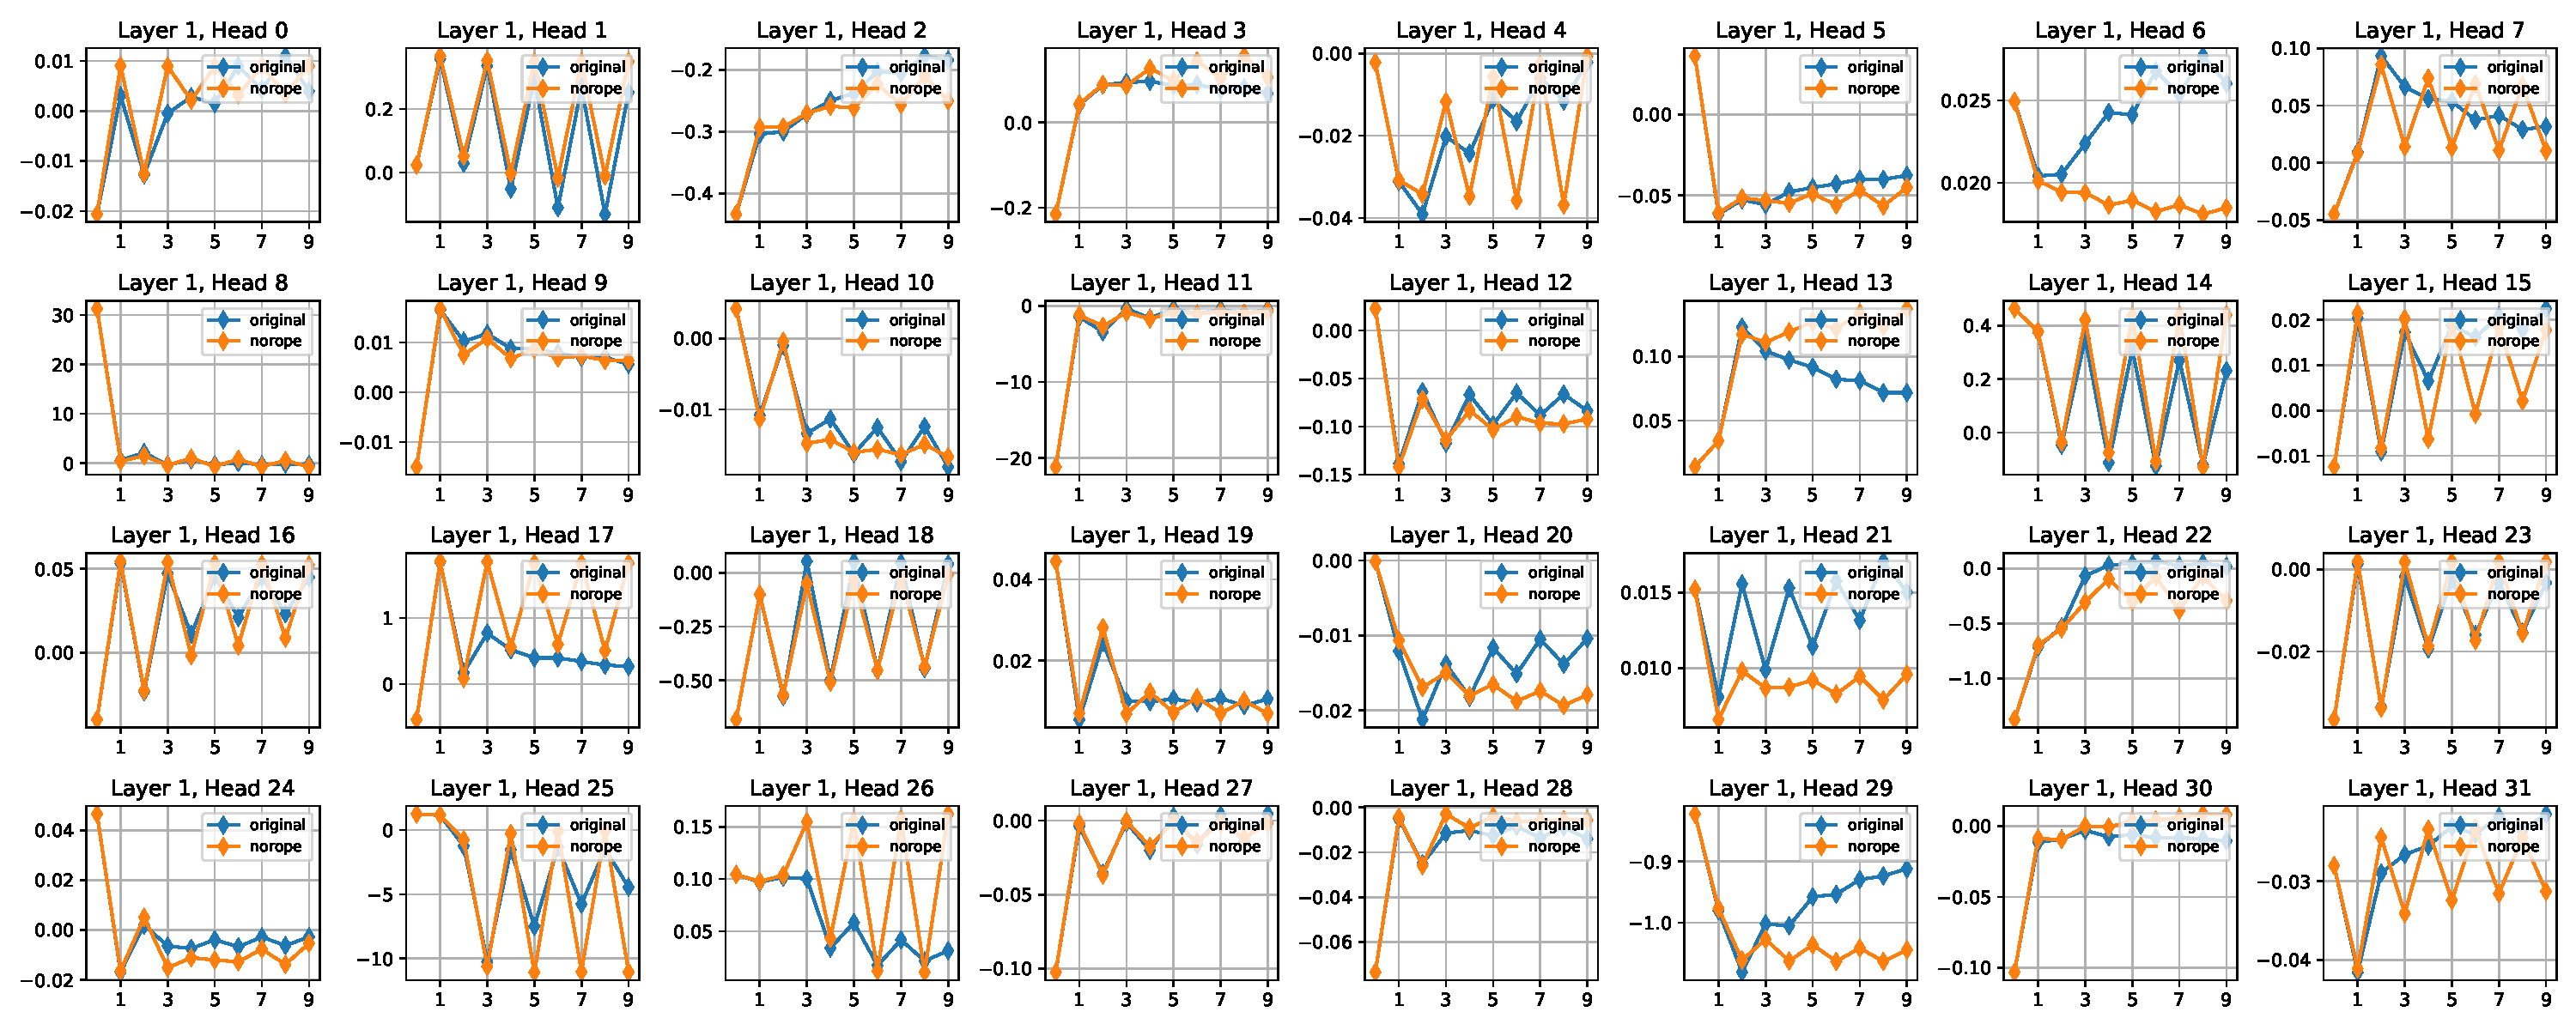
\includegraphics[width=\textwidth]{Figures/attn_0/attn_1_inner_prod_wstar.pdf}
    \caption{\small The inner product between $\Attn_1$'s \emph{OV output} in each head, and $\bw_\star$. We plot both across heads $m\in[M]$, and across tokens $\bh_i$ in the sequence. Sentence: ``Summer. Summer. Summer. Summer. Summer.'' We also consider a NoRoPE version where the RoPE in $\Attn_0$ is disabled. Observe that {\bf Head 8} produces a large output on the initial token.}
    \label{fig:attn1-heads-rope}
\end{figure}


\yub{Do we have an answer now for why initial token becomes massive? Based on Head 8}

\paragraph{Which head identifies delimiter tokens?}

When feeding LLM with a single token, the attention weights reduces to a point mass, and the attention output reduces to the summation of ``OV'' projections:
\begin{align}
    \Attn_0(\sets{\bh_0}) = \sum_{m=1}^M \bO_m\bV_m \bh_0, \quad \bO_m\in\R^{d\times (d/M)},~\bV_m\in\R^{(d/M)\times d}.
\end{align}

\begin{figure}[H]
    \centering
    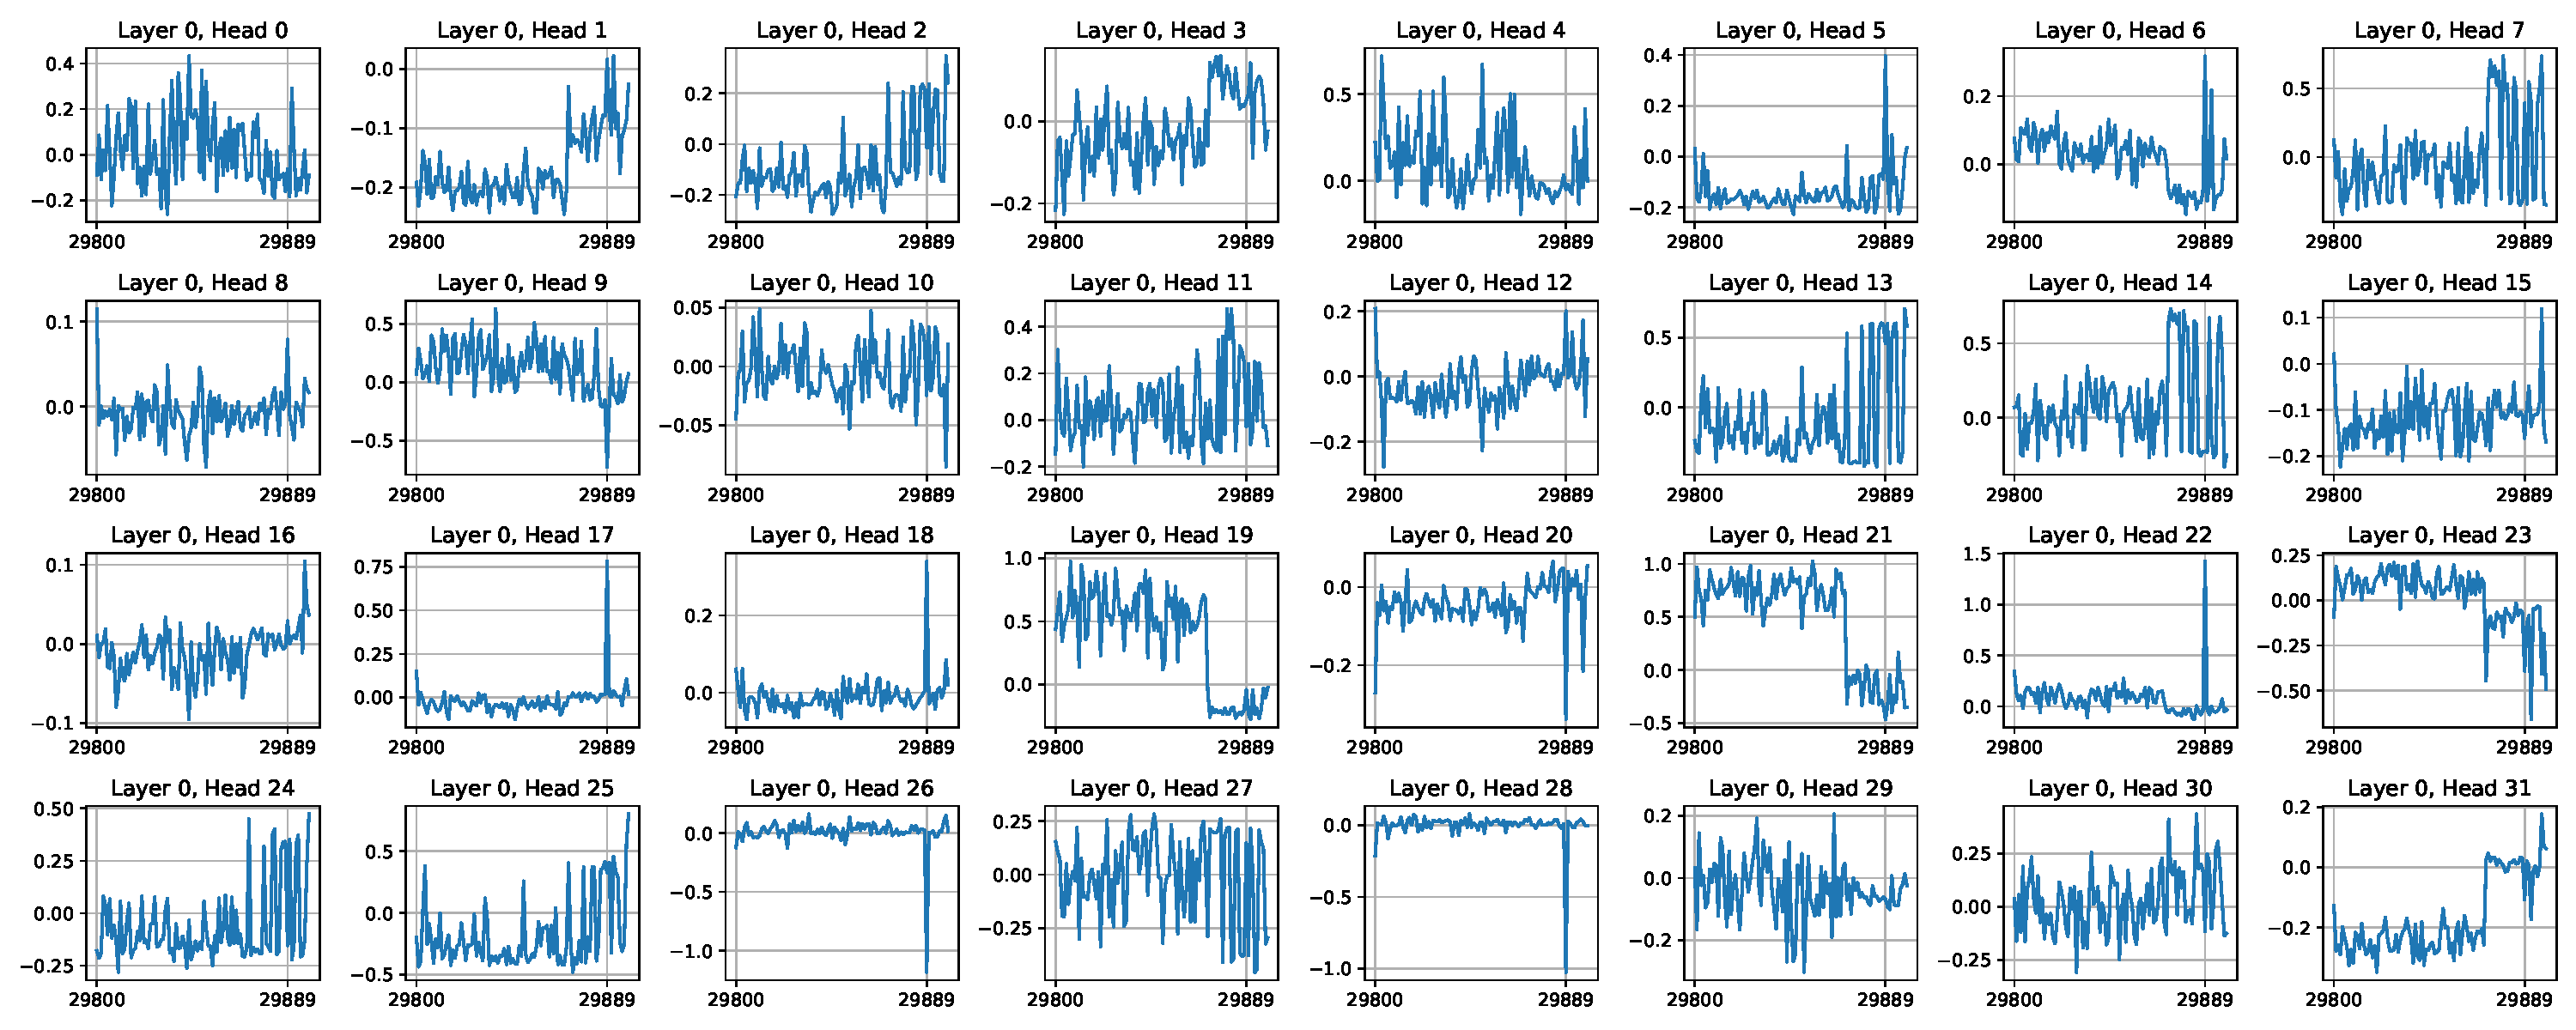
\includegraphics[width=\textwidth]{Figures/attn_0/attn_0_corr_wstar.pdf}
    \caption{\small The correlation of $\sets{\bO_m\bV_m\bh_0}_{m,\bh_0}\subset \R^d$ with $\bw_\star$ across both different heads $m\in[M]$, and across different tokens $\bh_0$ (corresponding to post-layernorm of the 32K token embeddings). Several heads identify the period token $29889$ (`.'). }
\end{figure}



\paragraph{Why the \emph{first} delimiter only?}
why does first delimiter become sink, and other layers not become sink?~\yub{TODO, some more symmetry breaking analysis with attention}

\begin{figure}[H]
    \centering
    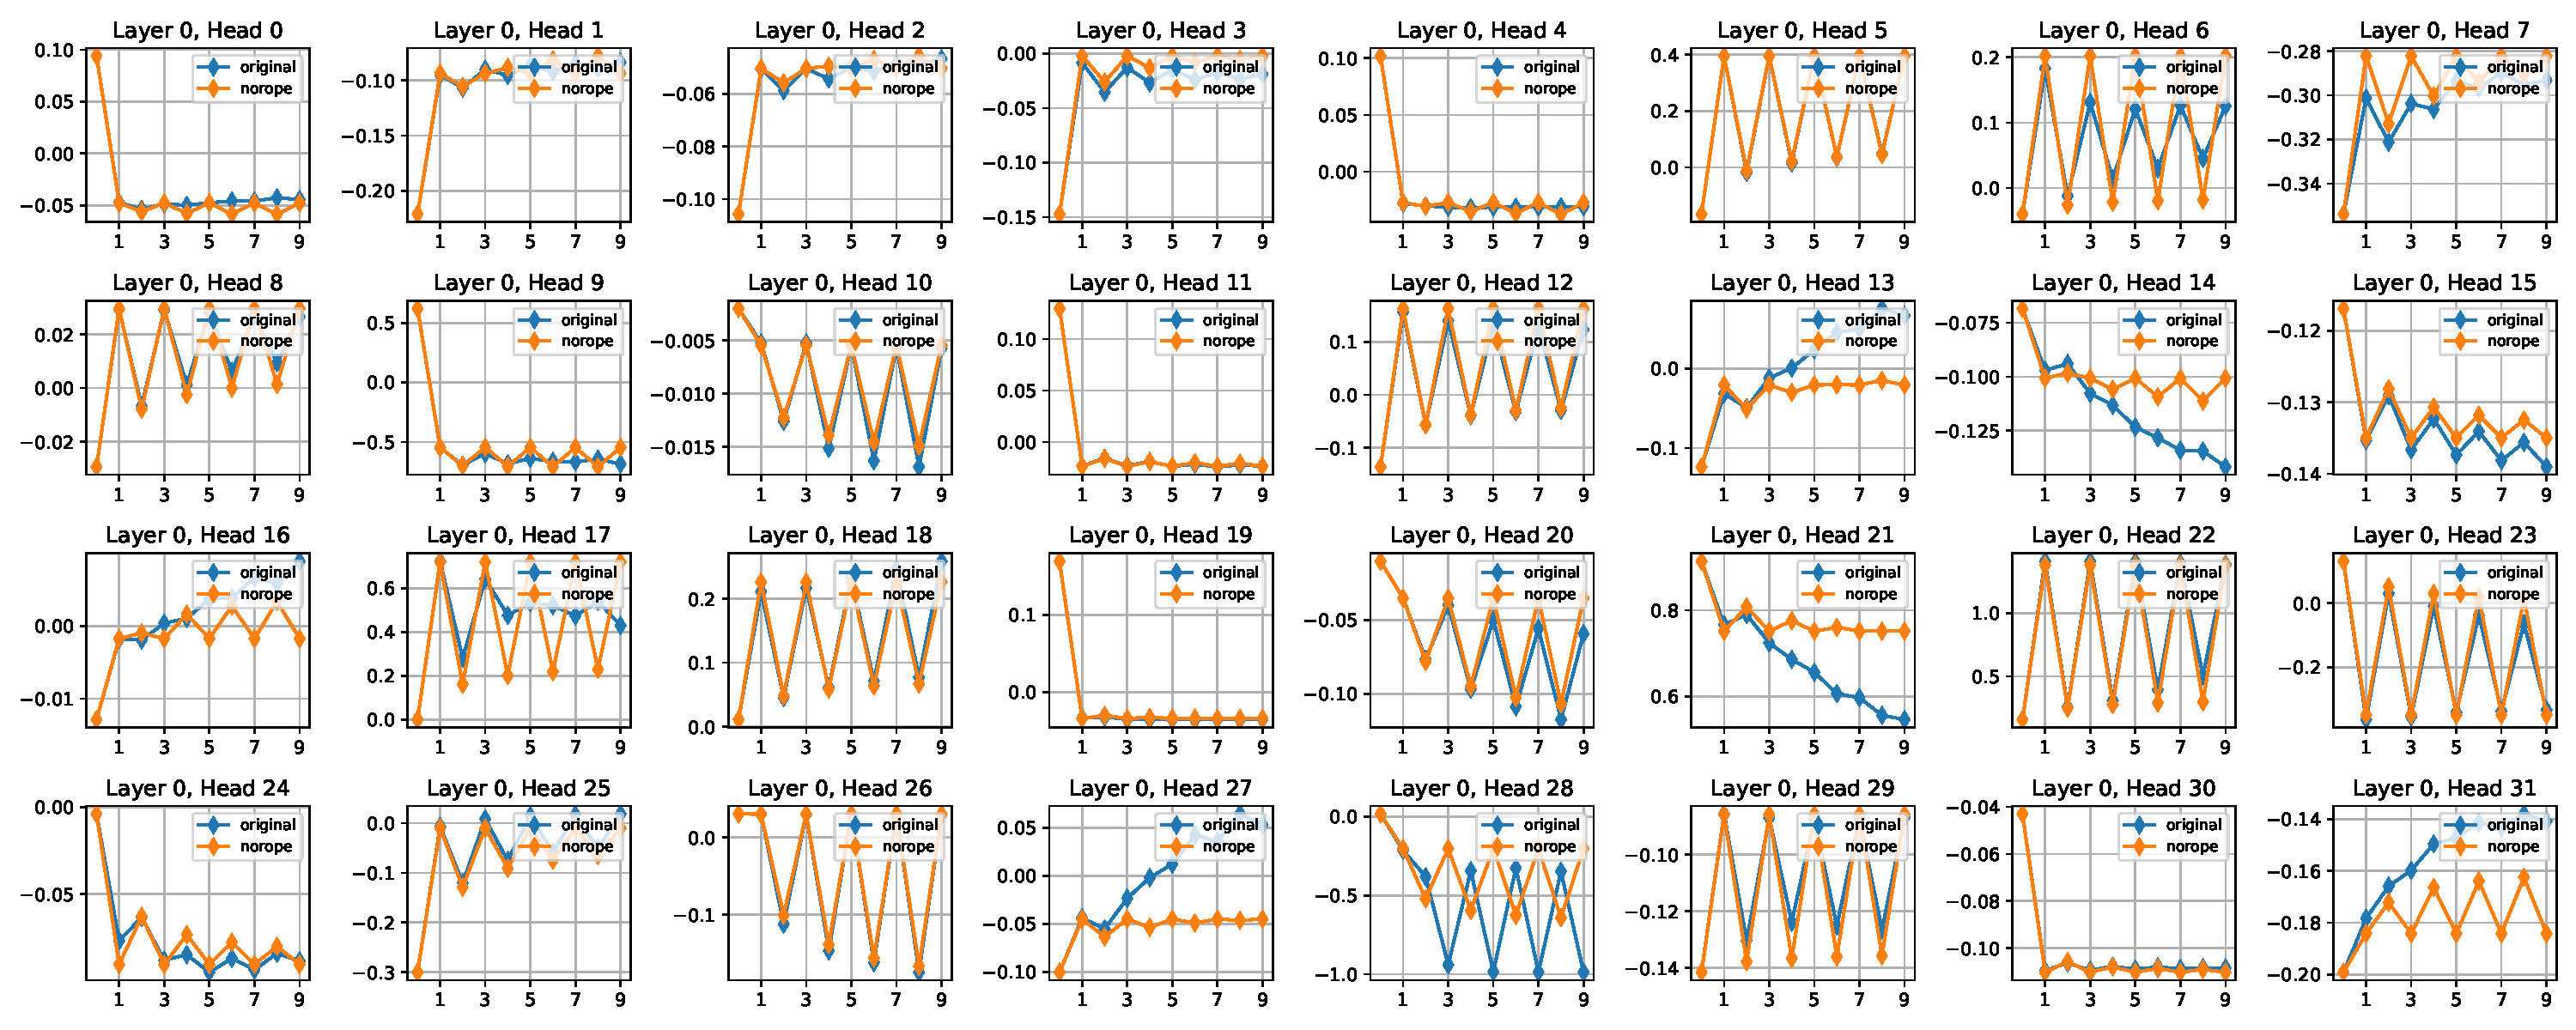
\includegraphics[width=\textwidth]{Figures/attn_0/attn_0_inner_prod_wstar.pdf}
    \caption{\small The inner product between $\Attn_0$'s \emph{OV output} in each head, and $\bw_\star$. We plot both across heads $m\in[M]$, and across tokens $\bh_i$ in the sequence. Sentence: ``Summer. Summer. Summer. Summer. Summer.'' We also consider a NoRoPE version where the RoPE in $\Attn_0$ is disabled. Observe that for {\bf Head 28}, the versions with and without RoPE differ significantly in their patterns.}
    \label{fig:attn0-heads-rope}
\end{figure}

% $w_\star^{(0)}=W_1^{(0)}[7374, :]$
Message: 1. We find, Head 28 in Attn 0 actually got impacted a lot by Rope. First, for period token, its OV state by head 28 produces a large negative correlation with $\bw_\star$ (see~\cref{fig:attn0-heads-rope}). Then, if there is rope in head 28 (as in regular LLM), then second period onward will attend significantly to prevoius period tokens. As a result, the attention output gives get large negative correlation. However, if there is no rope in head 28, then basiccally this negative correlation won't affect things, and period tokens would have positive correlation with $w_\star^{(0)}$. 

\begin{figure}[H]
\centering
\begin{minipage}{.32\textwidth}
\centering
    \subcaption{Attention weights of head 28 in layer 0}\label{fig:l0-h28-attn}
    %\vspace{-.7em}
    \includegraphics[width=0.95\textwidth]{Figures/tianyu_tentative/attn1 28.png}
\end{minipage}
% \hfill
\begin{minipage}{.32\textwidth}
\centering
    \subcaption{Cumulative correlations with $\bW_0[7374, :]$ across attention layer 0}\label{fig:attn-head-corr}
    %\vspace{-.7em}
    \includegraphics[width=0.95\textwidth]{Figures/tianyu_tentative/attn2 cum corr.png}
\end{minipage}
\begin{minipage}{.32\textwidth}
\centering
    \subcaption{Correlations between value states and $\bW_0[7374, :]$}\label{fig:value-corr}
    %\vspace{-.7em}
    \includegraphics[width=0.95\textwidth]{Figures/tianyu_tentative/values_w0star corr.png}
\end{minipage}
\caption{
\small
Mechanisms for the break of symmetry on the second delimiter.
}
\label{fig:special-neuron}
\vspace{-1em}
\end{figure}

\begin{figure}[H]
\centering
% \hfill
\begin{minipage}{.45\textwidth}
\centering
    \subcaption{Cumulative correlations with $\bW_1[7890, :]$ across attention layer 1}\label{fig:attn1-head-corr}
    %\vspace{-.7em}
    \includegraphics[width=0.95\textwidth]{Figures/tianyu_tentative/attn1 cum corr.png}
\end{minipage}
\begin{minipage}{.45\textwidth}
\centering
    \subcaption{Correlations between value states and $\bW_1[7890, :]$}\label{fig:value1-corr}
    %\vspace{-.7em}
    \includegraphics[width=0.95\textwidth]{Figures/tianyu_tentative/values w1star corrs.png}
\end{minipage}
\caption{
\small
Mechanisms for the break of symmetry on the second token.
}
\label{fig:special-neuron}
\vspace{-1em}
\end{figure}




The later mechanism in $\MLP_0$ and consequently $\MLP_1$ dictates that, a positive correaltion with $w_\star^{(0)}$ makes the token massive.


\subsection{Attention concentration}

\yub{Put initial plots + study in more depth.}

\subsection{Value anti-concentration}

\yub{Put initial plots + study in more depth.}

\subsection{Something else...?}

\yub{what happens for other architectures? Mainly mistral 7B.}

\yub{training dynamics? (can do this for either GPT2, or XGen-7B), for which we can obtain the model checkpoints.}